\documentclass[a4paper]{article}
    \usepackage[UTF8]{ctex}
    \usepackage{minted}
    \usepackage{xcolor}
    \usepackage[colorlinks,linkcolor=black]{hyperref}
    \usepackage[margin=1in]{geometry}
    \usepackage{caption}
    \usepackage{graphicx, subfig}
    \usepackage{float}
    \usepackage{fontspec}
    \setmainfont{Times New Roman}
    \setmonofont{Consolas}
    \definecolor{bg}{rgb}{0.9,0.9,0.9}
    \usemintedstyle{manni}
    \setminted{
    linenos,
    autogobble,
    breaklines,
    breakautoindent,
    bgcolor=bg,
    numberblanklines=false,
    }

\begin{document}
    \tableofcontents
    \newpage
    \section{实验介绍}
        \subsection{实验内容}
            \subsubsection{实验六}
使用web.py,结合前面学习的HTML,Lucene,中文分词等知识点,根据上次实验爬取的网页,建立一个简单的搜索引擎.搜索结果中要求包含:
标题,超链接,关键词上下文以及网址.
            \subsubsection{实验七}
制作一个图片加文字的搜索引擎,作为中期整合.即,在上次的基础上,加入图片搜索,使用css制定样式.

自主调节css中的各项属性参数与div布局,不存在标准答案,只需根据个人喜好决定页面表示形式和显示哪些细节.

        \subsection{实验环境}
操作系统:Ubuntu 18.04 LTS

Python版本:3.7

PyLucene版本:7.4.0

web.py版本:0.40.dev1
        \subsection{所需技能}
实验六主要涉及使用Python框架搭建简单的网站,用到了web.py,需要学习其基本的工作方式与API.同时,需要将之前实验中实现的多个功能模块,
如中文分词与Lucene索引,进行整合使用.

实验七主要在于整合前期工作,同时合理使用HTML和CSS布局来使得网页整齐美观.这一过程需要综合考虑多个模块,多次尝试调整,以达到满意的效果.
    \newpage
    \section{实验过程}
        \subsection{准备实验环境}
相较于之前的实验,本次实验仅需额外安装web.py即可准备好实验环境.但需要说明的是,由于web.py目前处于欠维护状态,其对Python 3的支持并非
十分完善.如果通过pip安装,需手动指定版本,否则所安装的版本将仅对Python 2可用:
\begin{minted}{bash}
pip install web.py==0.40-dev1
\end{minted}

更进一步的,由于我所使用的Python版本为最新的3.7,这样安装后的web.py依旧存在问题:框架报错而无法运行,静态文件访问出错等.这些问题主要是
由于Python 3.7的一些变动导致的,为解决这些问题,需要手动从Github上下载最新的web.py源码安装,如下:
\begin{minted}{bash}
git clone git://github.com/webpy/webpy.git
ln -s `pwd`/webpy/web .
\end{minted}
        \subsection{后端构建}
            \subsubsection{设置JVM与Lucene}
由于PyLucene仅仅是Lucene的Python接口,Lucene本身是运行于Java虚拟机环境(JVM)中,需要在Python程序中启动JVM,并且在每次执行
搜索时调用.对于web.py,在主程序中启动Web应用时,会将当前所有的全局变量,即\mintinline{python}{globals()},打包传递给web.py程序,
并且在之后的每次响应时从中获取所需变量.

那么,我们需要在主程序中启动JVM,作为全局变量供之后使用.同时,为了避免每次搜索时创建Lucene搜索器的开销,可以在程序启动时
就创建好搜索器,同样作为全局变量传递.如下:
\begin{minted}{python}
if __name__ == '__main__':
    vm_env = lucene.initVM(vmargs=['-Djava.awt.headless=true'])
    base_dir = os.path.dirname(os.path.abspath(sys.argv[0]))
    directory = {
        "html": SimpleFSDirectory(Paths.get(os.path.join(base_dir, HTML_INDEX_DIR))),
        "image": SimpleFSDirectory(Paths.get(os.path.join(base_dir, IMAGE_INDEX_DIR))),
    }
    searcher = {
        "html": IndexSearcher(DirectoryReader.open(directory["html"])),
        "image": IndexSearcher(DirectoryReader.open(directory["image"])),
    }
    analyzer = StandardAnalyzer()
    app = web.application(urls, globals(), autoreload=False) #attention here
    app.run()
\end{minted}

注意在上面的代码中,需要禁用web.py的自动重载,否则会导致上述代码失效.可能的原因在于此种情况下主程序将不再是我们编写的
该文件,而是web.py自身,则\mintinline{python}{__name__!='__main__'},而是实际的文件名.

在初始化JVM后,只需在每次调用时:
\begin{minted}{python}
vm_env.attachCurrentThread()
\end{minted}
            \subsubsection{设置路由}
由于需要区分网页搜索和图片搜索(当然也可以不区分,只需在搜索时额外传递一个类型参数),则对二者的Index页面各自分配一个处理类(原因在于
这两个类都非常简洁),但对于搜索结果页面,我选择共用一个类,通过URL来区分类别(原因在于处理网页和图片的搜索请求流程基本相同,可以
通过共用类来减少冗余代码).如下:
\begin{minted}{python}
urls = (
    "/", "Index",
    "/image", "IndexImage",
    "/search/(.+)", "Search",
)

class Index:
    def GET(self):
        return render.index()

class IndexImage:
    def GET(self):
        return render.index_image()

class Search:
    def GET(self, search_type="html"):
        search_data = web.input()
        query_string = search_data.get("s", "")
        if search_type not in ("html", "image"):
            search_type = "html"
        if not query_string:
            return render.index_image() if search_type == "image" else render.index()
        search_result = search_function[search_type](query_string)
        return result_template[search_type](query_string, search_result)
\end{minted}

注意以上代码的最后两行,通过表驱动法避免了if-else语句的泛滥,对于目前仅有的两种搜索类型可能优势并不明显,但可以方便地添加
新的搜索类型而无需修改此处逻辑,有利于日后的功能增加.
        \subsubsection{网页搜索}
对网页的搜索,在往次实验的基础上,只需对原有程序作出一些修改,即可基本实现,故不再此赘述.
主要的问题在于,如何实现关键词上下文以及关键词高亮.

让我们稍做分析:Lucene所创建的索引中,并未保存网页的完整内容(\mintinline{python}{t.setStored(False)}),
而是对其进行提取处理后保存了索引信息(如倒排索引).那么,自然是难以通过Lucene直接对关键词进行高亮处理,除非重新创建索引
并且保存网页的内容信息.

那么,我采用了十分朴素的高亮方式:打开检索结果对应的本地HTML文件,对其内容进行去HTML标签及分词处理,得到一个词汇列表,然后将其与
输入的搜索字符串分词后的词汇列表对比,找到第一个重合项,然后将此项的前后一定数量的词汇合并为所展示的内容摘要.如下:
\begin{minted}{python}
with open(doc.get("path"), mode="r", encoding="utf8") as file:
    content = file.read()
html2text = HTML2Text()
html2text.ignore_links = True
html2text.ignore_images = True
content = html2text.handle(content)
cutted_content = jieba.cut(content)
flag = False
if cutted_query:
    word_num, cnt = 20, 0
    for x in cutted_content:
        if not x.strip():
            continue
        if not flag and x in cutted_query:
            flag = True
            content = ""
        if flag and cnt < word_num:
            cnt += 1
            content += (x if x not in cutted_query else
                        "<span class='highlight'>{0}</span>".format(x)
                        )
        elif cnt >= word_num:
            break
single_result["content"] = content if flag else content[:100]
\end{minted}

这样的做法可能有些粗糙,但效果尚可接受,在后续的实验中,必要时需要对其做出修改.
            \subsubsection{图片搜索}
类似的,图片搜索基本上可以利用之前实验的代码实现,仅需做出一些简单的修改.
\begin{minted}{python}
def search_image(query_string, result_num=10):
    vm_env.attachCurrentThread()
    cutted = [x for x in jieba.cut_for_search(query_string) if x.strip()]
    command = " ".join(cutted)
    query = QueryParser("content", analyzer).parse(command)
    scoreDocs = searcher["image"].search(query, result_num).scoreDocs
    result = list()
    for num, scoreDoc in enumerate(scoreDocs):
        doc = searcher["image"].doc(scoreDoc.doc)
        single_result = {
            "url": doc.get("url"),
            "description": doc.get("raw_content"),
        }
        result.append(single_result)
    return result
\end{minted}
        \subsection{前端构建}
            \subsubsection{Index页面}
网页搜索的Index页面主体部分都是一个文本输入框加上表单提交的按键.为了使网页整齐,使用CSS+DIV进行布局:
\begin{minted}{HTML}
<!DOCTYPE html>
<html lang="zh">
<head>
    <meta charset="UTF-8">
    <link rel="stylesheet" href="/static/css/main.css">
    <title>网页搜索</title>
</head>
<body>
    <div id="magicWrapper">
    <div id="superCenter" align="center">
        <h1 style="font-size: 60px;" >
            <span>The</span><span class="beacon">Beacon</span>
        </h1>
        <div id="searchType">
            <span class="active"><a href="/">网页</a></span>
            <span class="type"><a href="/image">图片</a></span>
        </div>
        <div id="homeSearch" align="center">
            <form action="/search/html">
                <input type="text" id="homeInput" name="s" placeholder="搜点什么吧">
                <input type="submit" id="homeSubmit" value="搜索">
                <br>
            </form>
        </div>
    </div>
    </div>
</body>
</html>
\end{minted}

具体的CSS属性不在此贴出,最终实现的效果如下:
\begin{figure}[H]
\centering
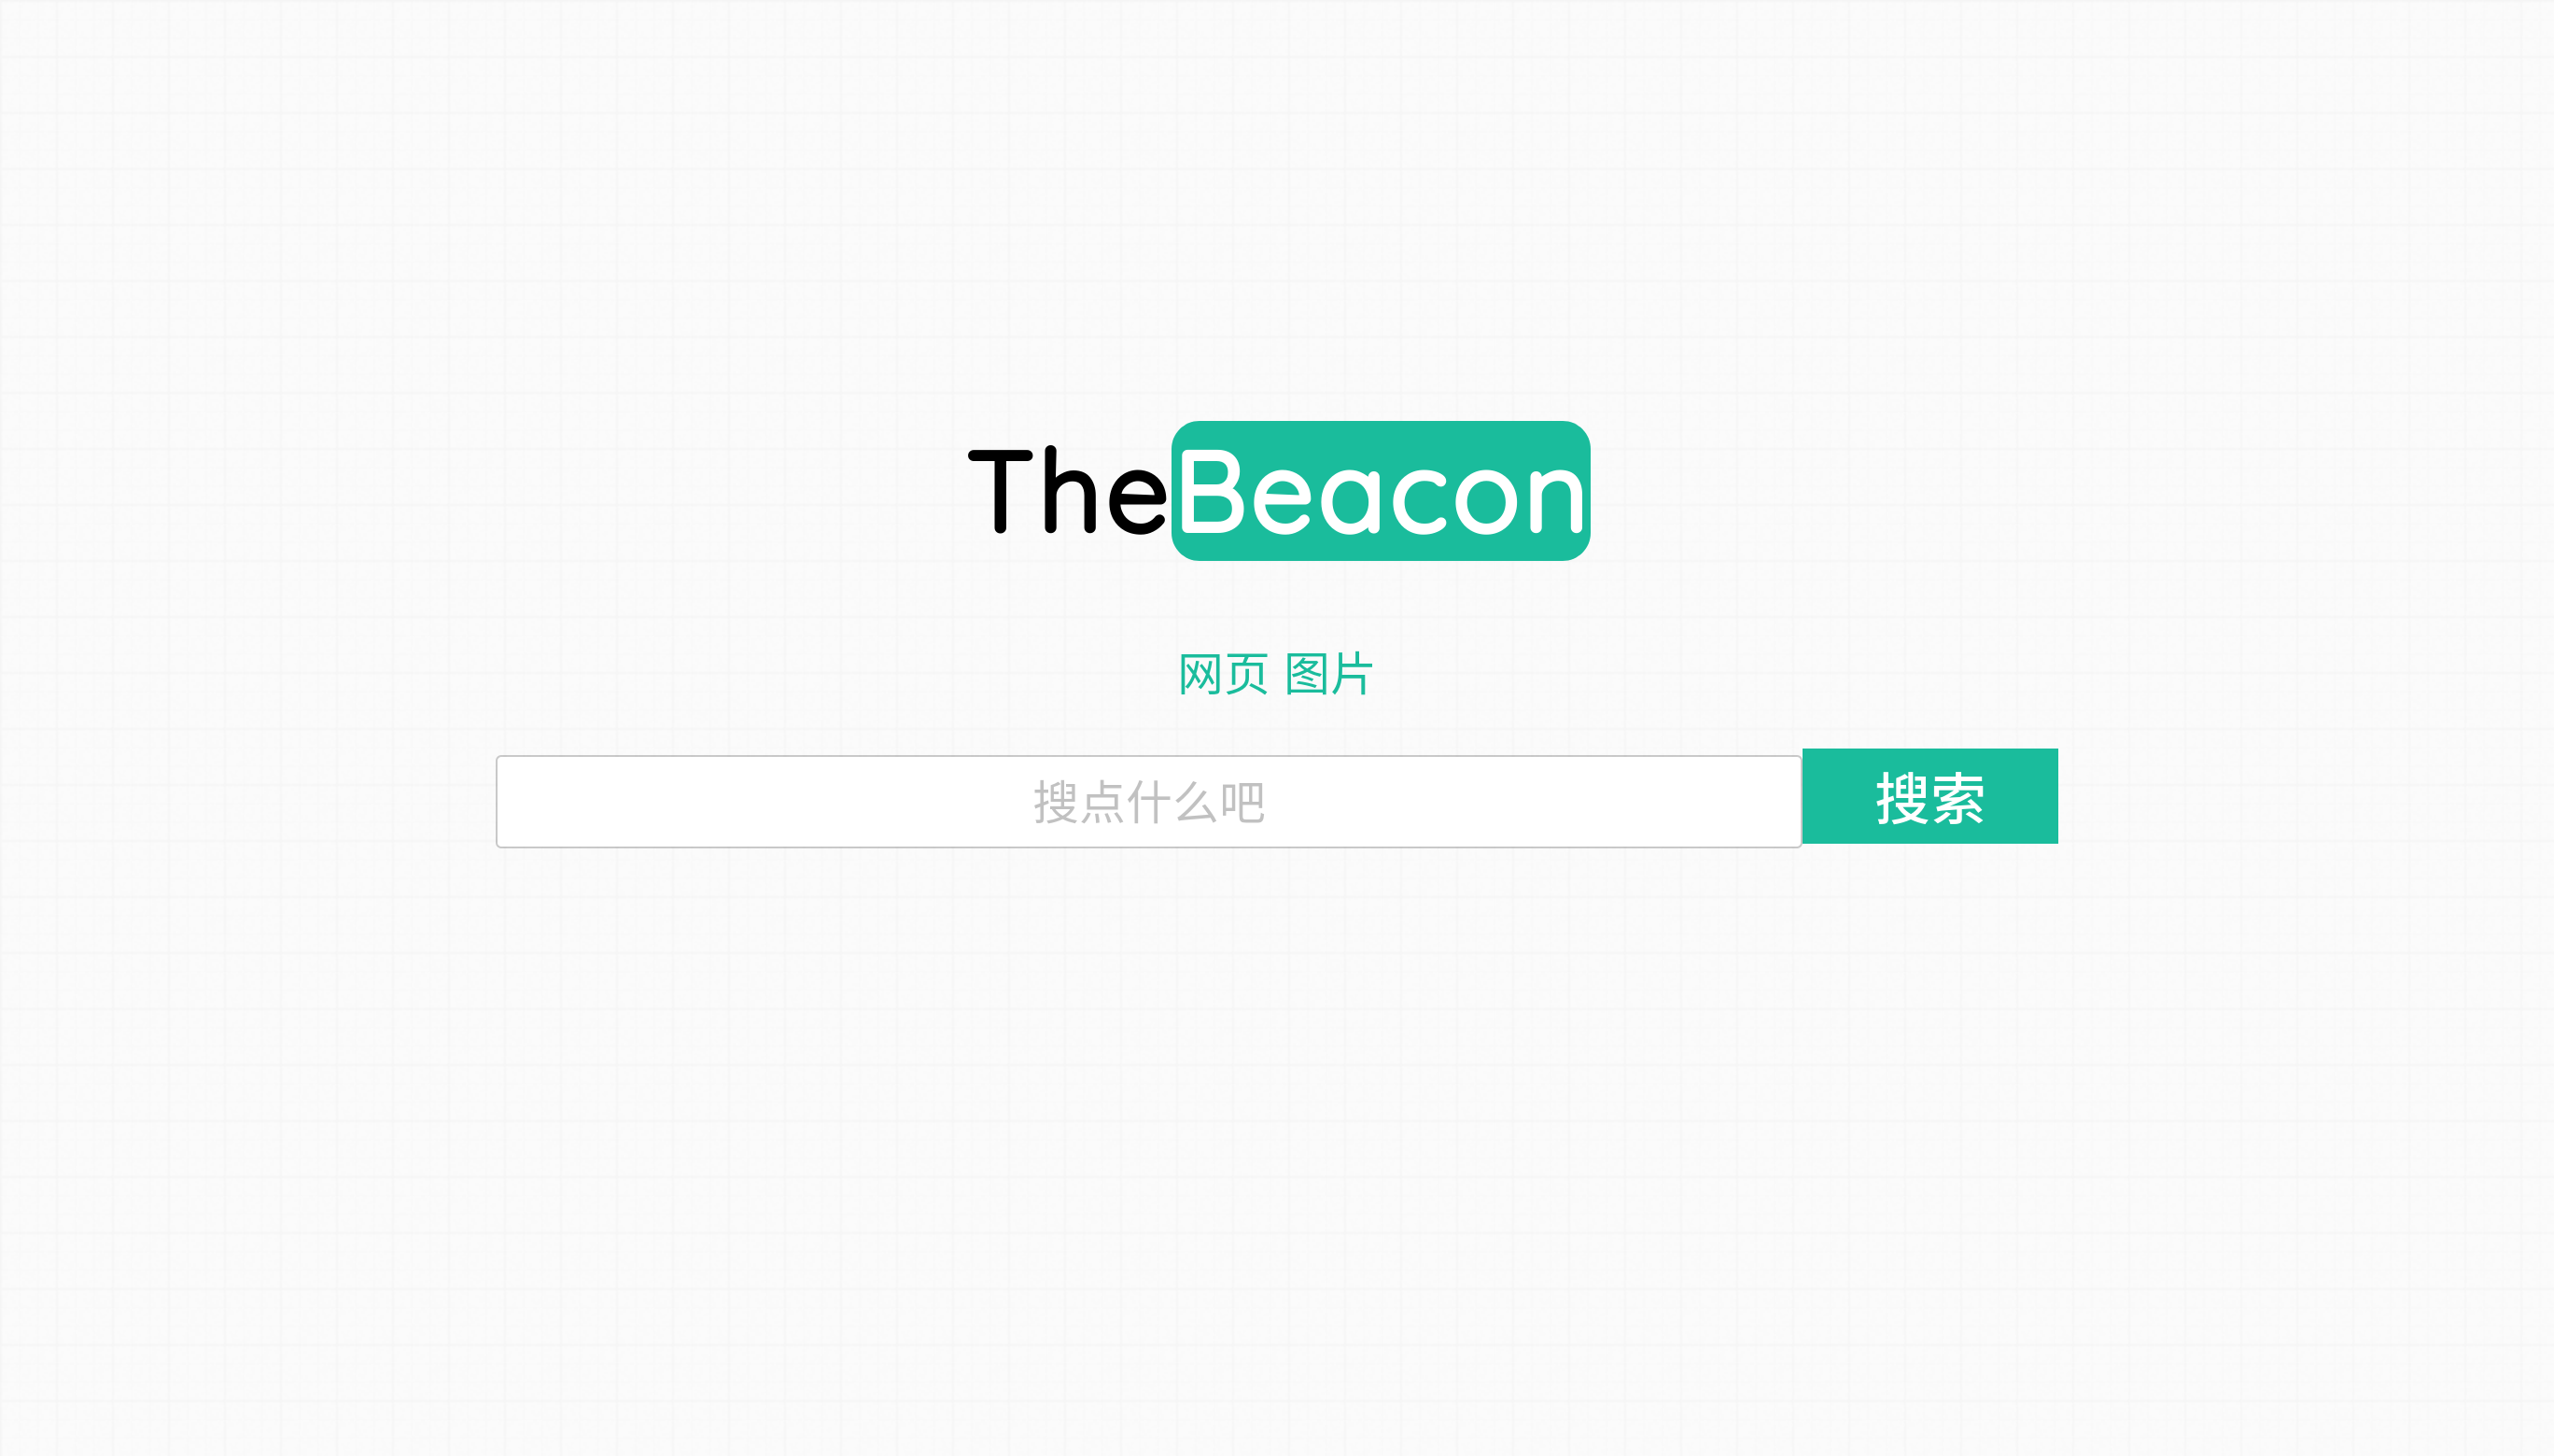
\includegraphics[width=\textwidth]{img/index.png}
\caption{网页搜索Index页面}
\end{figure}

而对于图片搜索,其布局基本类似,为了体现图片搜索的特点而有所区分,对其设置了不同的背景,效果如下:
\begin{figure}[H]
\centering
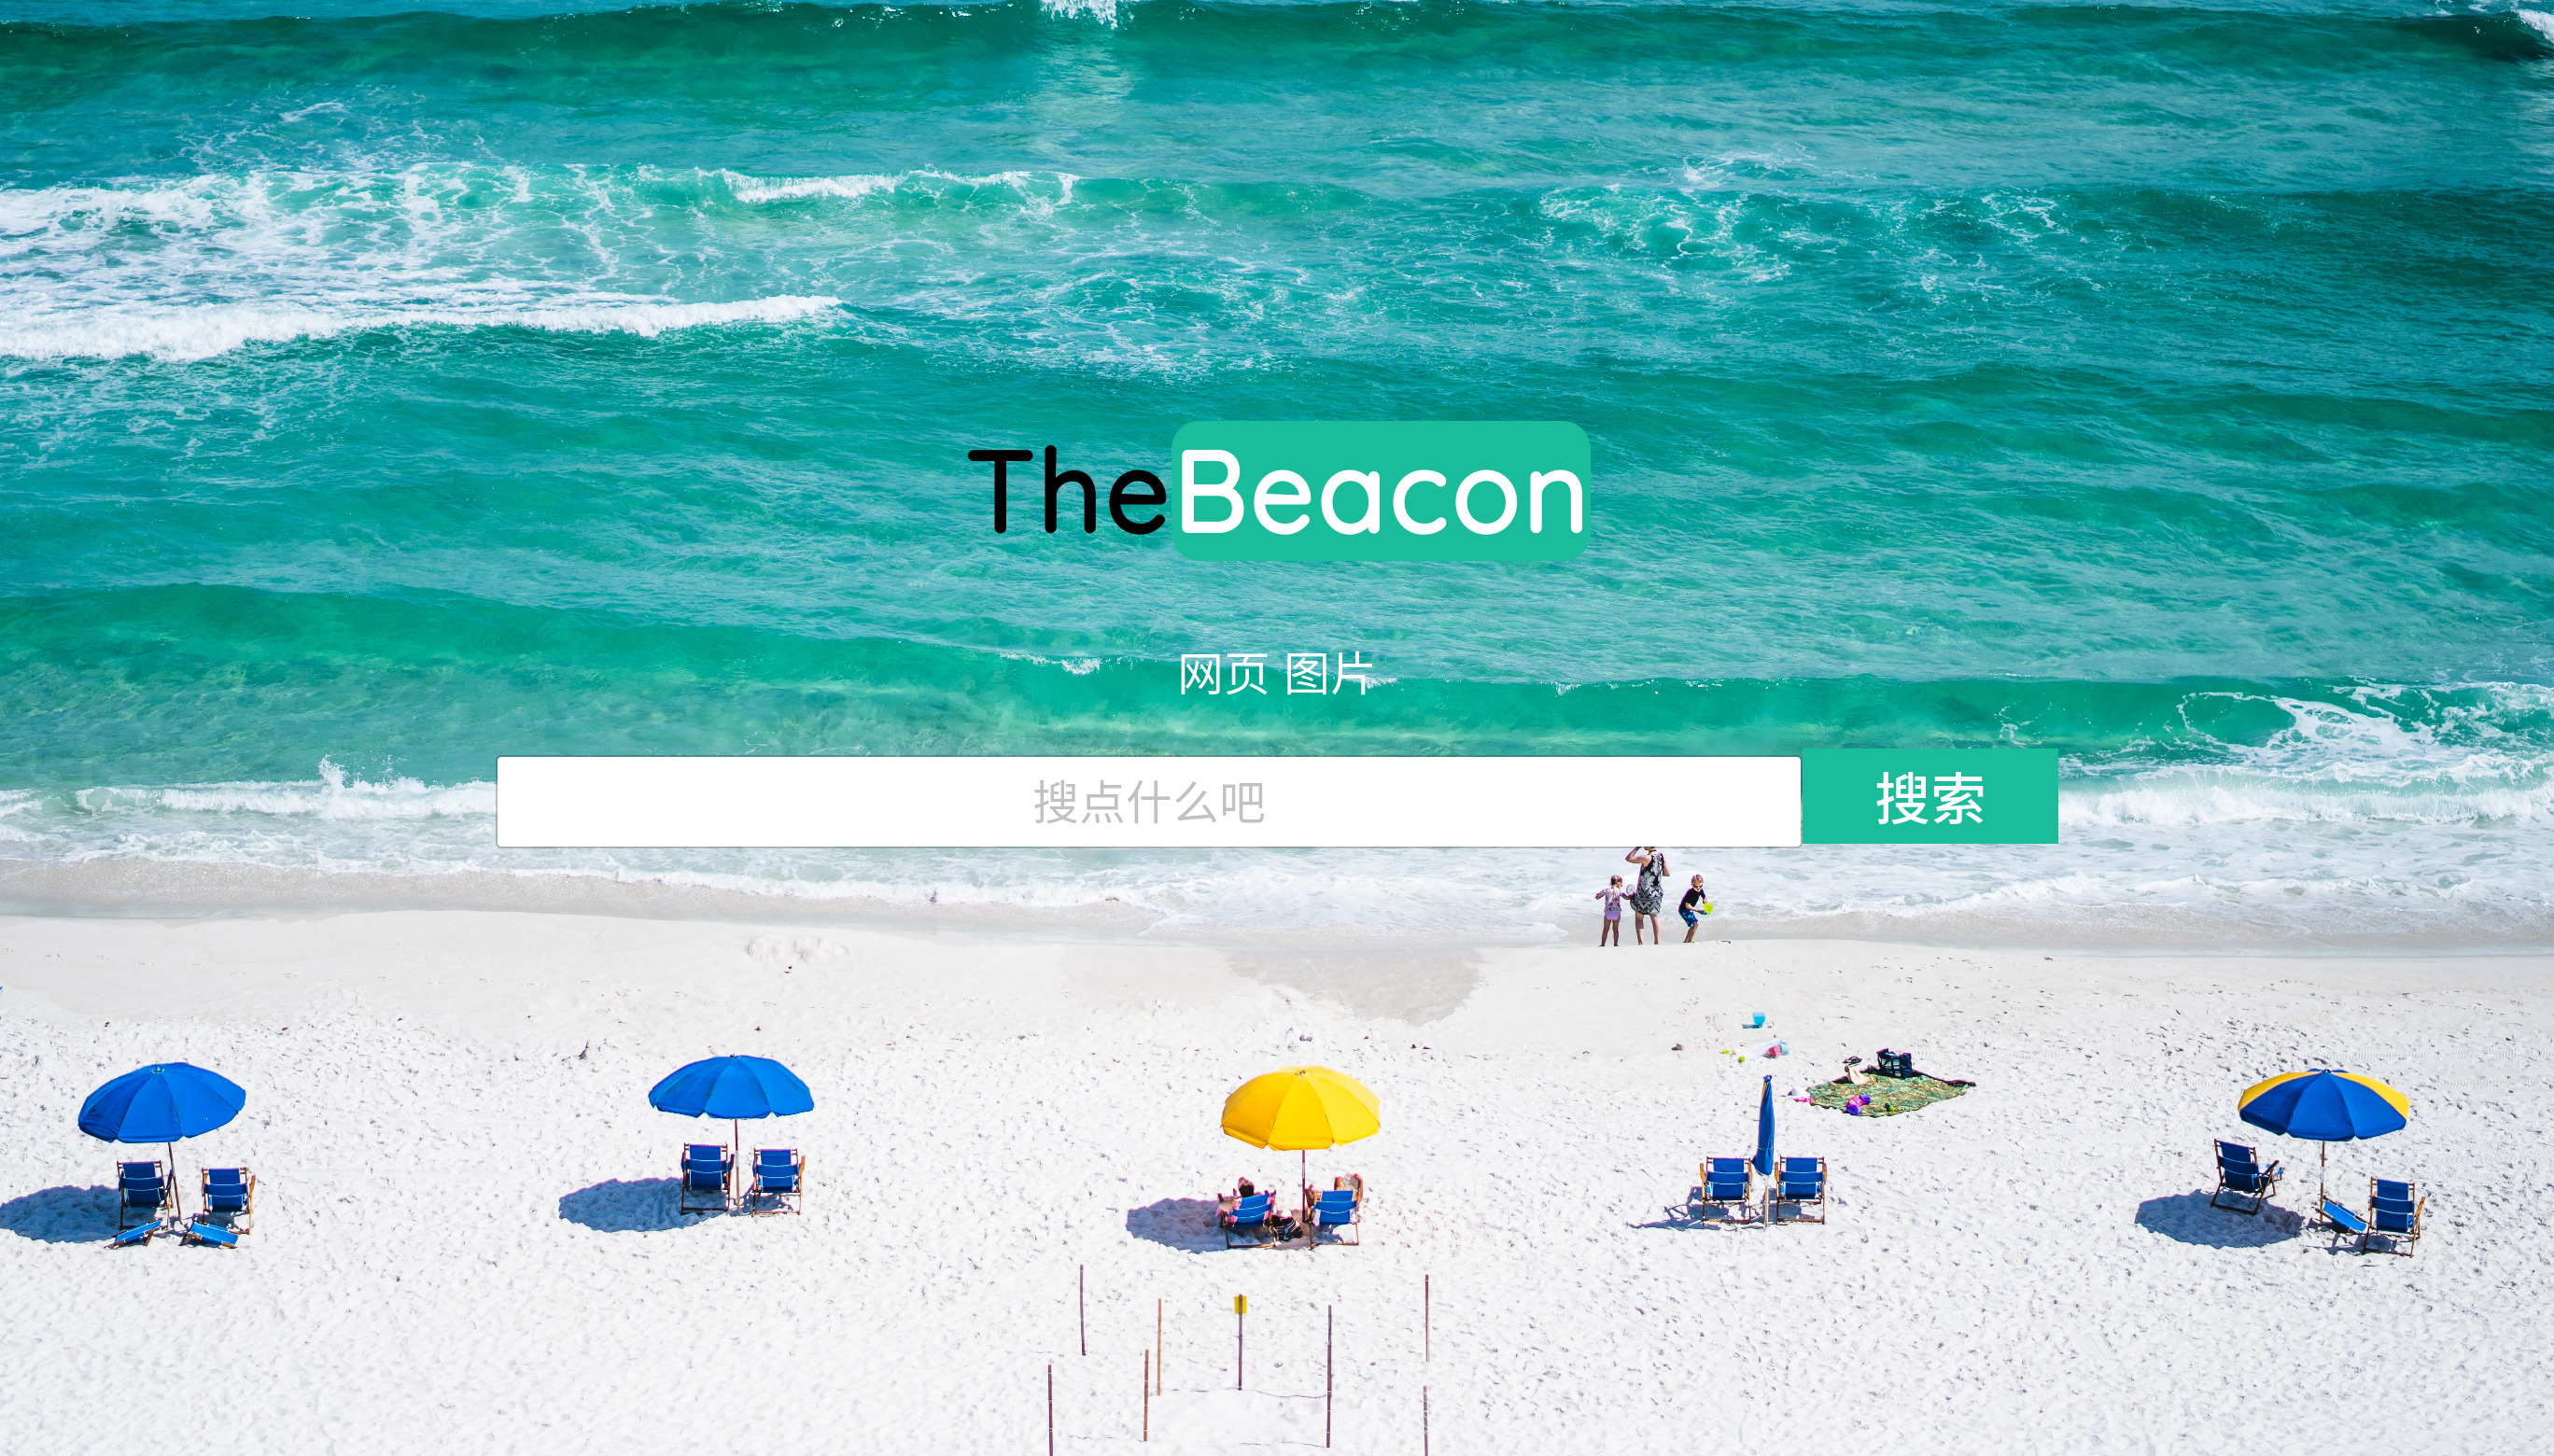
\includegraphics[width=\textwidth]{img/index_image.jpg}
\caption{图片搜索Index页面}
\end{figure}
            \subsubsection{网页搜索结果页面}
搜索结果页面模板接受Python传来的参数:\mintinline{python}{query_string,search_result},类型分别为字符串以及字典组成的列表,
以此生成搜索页面.则可布局为多个DIV,每个DIV为一条搜索结果.同时,为了方便使用,可以设置一个始终悬浮于页面最上的输入框,用于进行新的
搜索.
\begin{minted}{html}
$def with (query_string,search_result)
<!DOCTYPE html>
<html lang="zh">
<head>
    <meta charset="UTF-8">
    <link rel="stylesheet" href="/static/css/main.css">
    <title>$query_string 网页搜索结果</title>
</head>
<body>
    <div class = "floatingBar">
        <form action="/search/html">
            <input type="text" name="s" class="floatingInput" value= "$query_string">
            <input type="submit" class="floatingSubmit" value="搜索">
        </form>
    </div>
    <div class = "resultContainer">
        $for item in search_result:
        <div class = "item">
            <div class = "title">
                <a href="$item['url']">$item["title"]</a>
            </div>
            <div class = "content">$:item["content"]</div>
            <div class = "url">
                <a href="$item['url']">$item["url"][:80]</a>
            </div>
        </div>
    </div>
</body>
</html>
\end{minted}

用到的主要CSS属性如下:
\begin{minted}{CSS}
div.item{
    margin-bottom: 10px;
    padding: 20px 15px 15px;
    border-radius: 5px;
    background-color: #fff;
    box-sizing: border-box;
    box-shadow: 0 0 20px 2px rgba(0, 0, 0, .1);
    -webkit-box-shadow: 0 0 20px 2px rgba(0, 0, 0, .1);
    -moz-box-shadow: 0 0 20px 2px rgba(0, 0, 0, .1);
}


.floatingBar{
    position: fixed;
    top: 10px;
    width:80%;
    margin-left: 10%;
    margin-right: 10%;
}
\end{minted}

最终效果如图所示:
\begin{figure}[H]
\centering
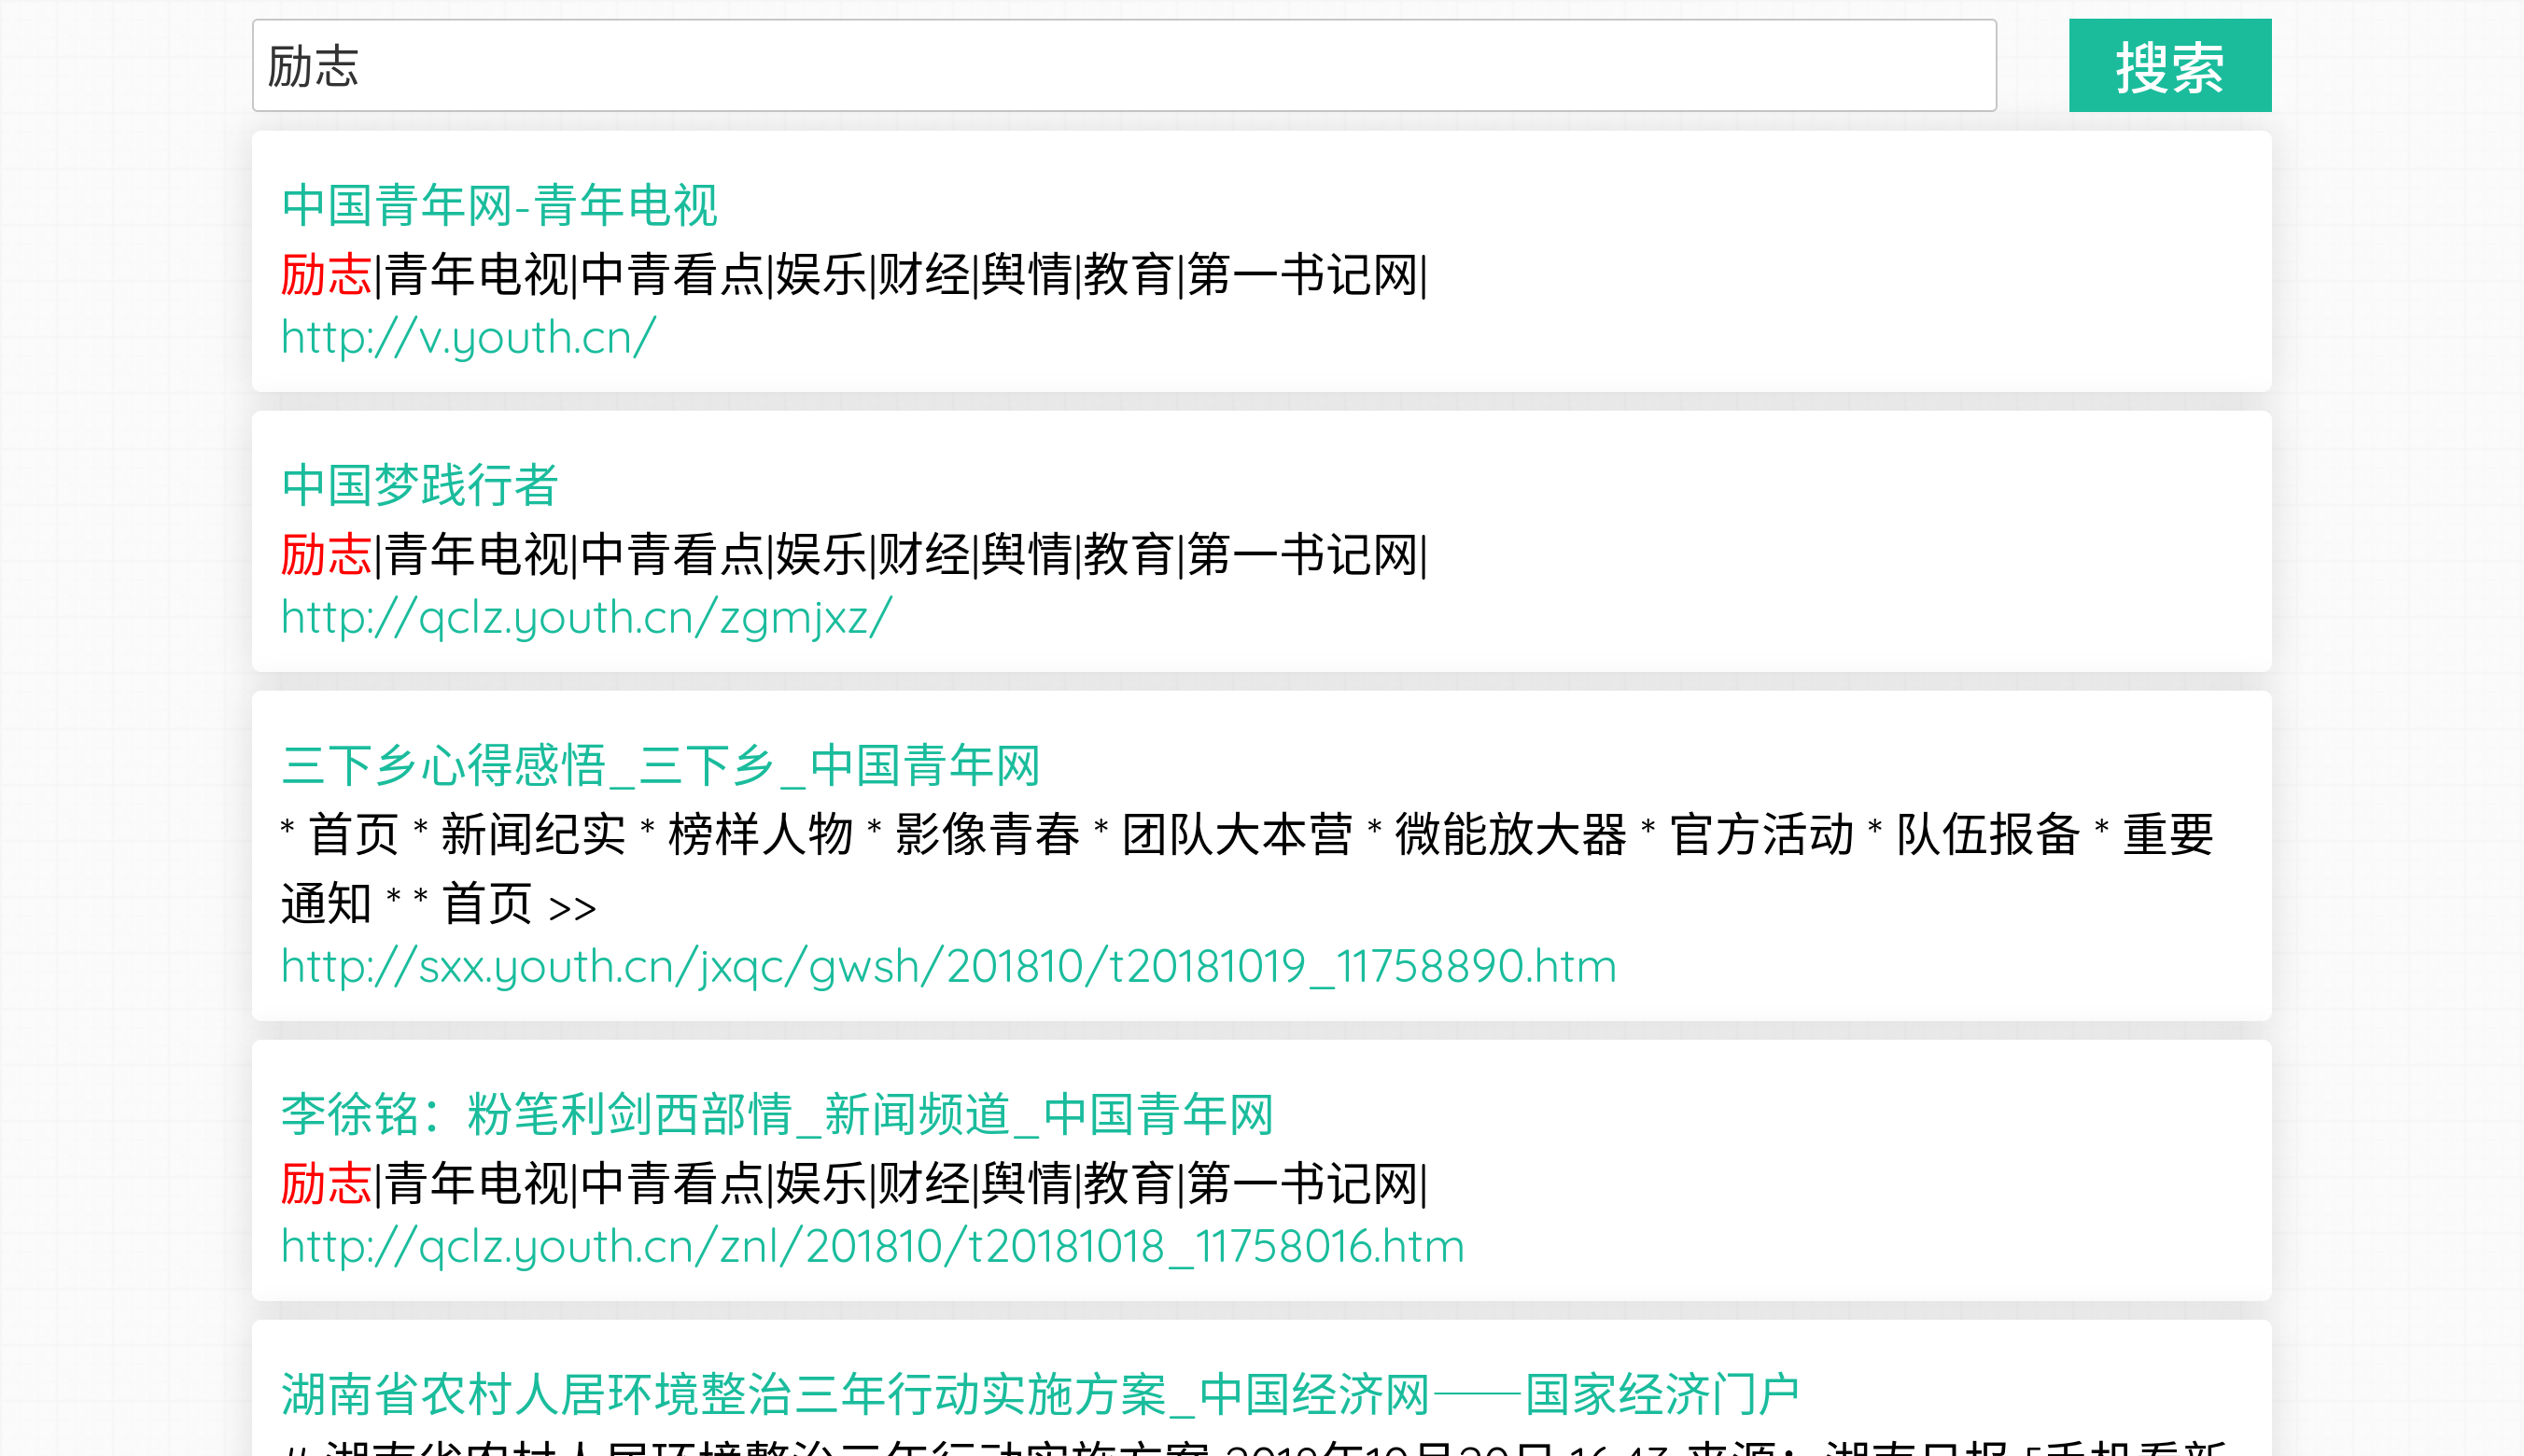
\includegraphics[width=\textwidth]{img/result.png}
\caption{网页搜索结果}
\end{figure}
        \subsubsection{图片搜索结果页面}
对于图片的搜索结果,每张图片都配有一定的描述文字,可将其放在一个DIV中,然后对所有的DIV进行排列.一种比较美观
的排列方式为瀑布流,这部分的CSS布局代码参考了网上的代码.\footnote{https://blog.csdn.net/m0\_37568521/article/details/78487568}

则HTML模板的主要部分形如:
\begin{minted}{html}
<div class = "waterfall">
    $for item in search_result:
    <div class = "item">
        <img src="$item['url']">
        <div class = "url">$item["description"][:80]</div>
    </div>
</div>
\end{minted}

最终效果如下:
\begin{figure}[H]
\centering
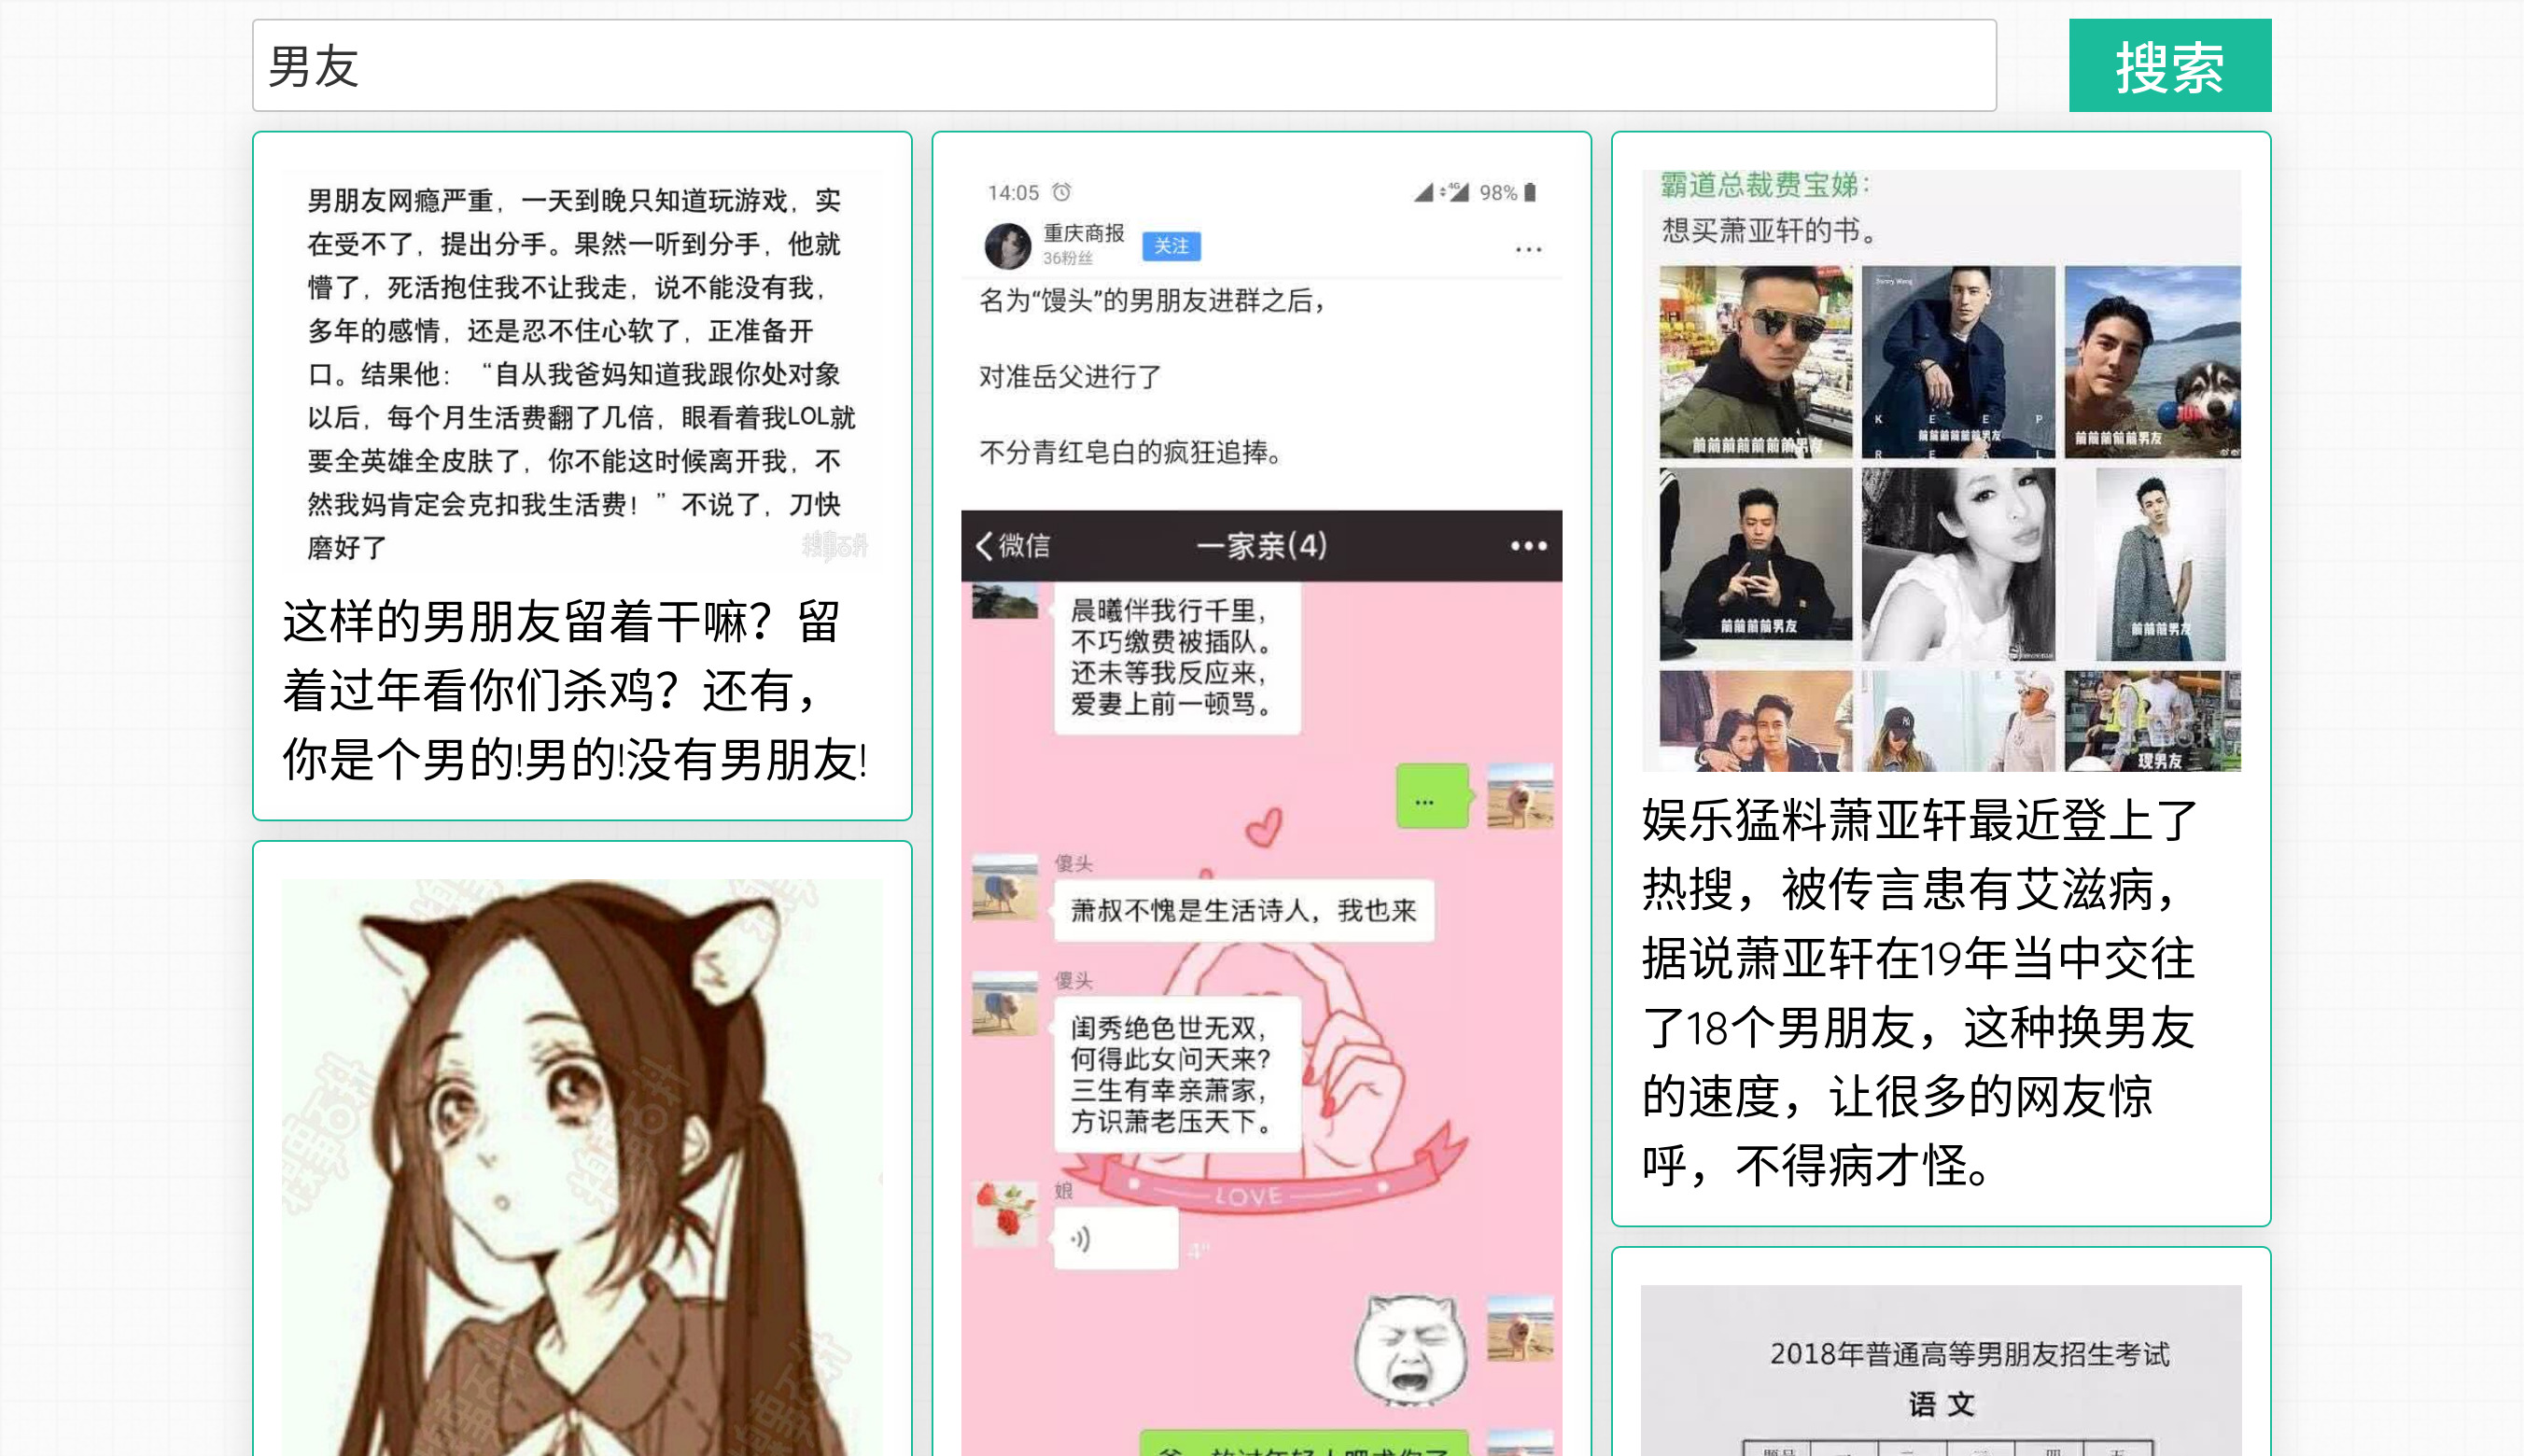
\includegraphics[width=\textwidth]{img/result_image.jpg}
\caption{图片搜索结果}
\end{figure}
\newpage
    \section{总结与分析}
本次实验将之前实验内容进行了整合,在这一过程中,我发现了以前所写代码的一些缺陷,诸如不能灵活配置参数,过度依赖上下文等,
这些都阻碍着对其的整合.因此,在今后的编程中,更需要注意模块化的设计思想.

此外,在编写HTML和CSS代码时,由于没有正式地学习过前端知识,常常遇到一些难以处理的细节问题,需要反复尝试并查找各种资料,
耗费了不少时间,但也加深了对其的理解与掌握.
\end{document}
